\documentclass[]{standalone}

\usepackage[dvipsnames]{xcolor}
\usepackage{amsmath}
\usepackage{tikz}
\usetikzlibrary{calc}
\usetikzlibrary{tikzmark}


\newcommand*\circled[1]{\tikz[baseline=(char.base)]{
            \node[shape=circle,draw,inner sep=2pt] (char) {#1};}}
            
            
\begin{document}
\renewcommand{\arraystretch}{1.5}
\renewcommand{\tabcolsep}{10pt}
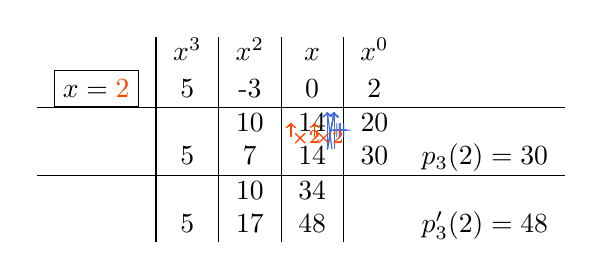
\begin{tikzpicture}[remember picture]
\node at (0,0) {
\begin{tabular}{c|c|c|c|cc}
 & $x^3$ & $x^2$ & $x$ & $x^{0}$\\
$\boxed{x=\textcolor{OrangeRed}{2}}$ & \subnode{A}{5} & \subnode{B}{-3} & \subnode{C}{0} & \subnode{D}{2}\\\hline
 & & \subnode{L}{10} & \subnode{M}{14} & \subnode{N}{20}\\
 & \subnode{E}{5} & \subnode{F}{7} & \subnode{G}{14} & \subnode{H}{30} & $p_3(2)=30$\\\hline
 & & \subnode{O}{10} & \subnode{P}{34}\\
 & \subnode{I}{5} & \subnode{J}{17} & \subnode{K}{48} & & $p_3'(2)=48$\\
\end{tabular}};
\def\spacing{2.5mm}
\draw[->, RoyalBlue] (A.south)+(\spacing,0) -- ($(E.north)+(\spacing,0)$) node[midway,inner sep=0.2pt, anchor=west] {\scriptsize +};
\draw[->, RoyalBlue] (B.south)+(\spacing,0) -- ($(F.north)+(\spacing,0)$) node[midway,inner sep=0.2pt, anchor=west] {\scriptsize +};
\draw[->, RoyalBlue] (C.south)+(\spacing,0) -- ($(G.north)+(\spacing,0)$) node[midway,inner sep=0.2pt, anchor=west] {\scriptsize +};
\draw[->, RoyalBlue] (D.south)+(\spacing,0) -- ($(H.north)+(\spacing,0)$) node[midway,inner sep=0.2pt, anchor=west] {\scriptsize +};

\draw[->, shorten <= -1mm, shorten >= -1mm, OrangeRed] (E) -- (L) node[midway,anchor=north west, inner sep=0pt] {\scriptsize $\times 2$};
\draw[->, shorten <= -1mm, shorten >= -1mm, OrangeRed] (F) -- (M) node[midway,anchor=north west, inner sep=0pt] {\scriptsize $\times 2$};
\draw[->, shorten <= -1mm, shorten >= -1mm, OrangeRed] (G) -- (N) node[midway,anchor=north west, inner sep=0pt] {\scriptsize $\times 2$};

\draw[->, RoyalBlue] (E.south)+(\spacing,0) -- ($(I.north)+(\spacing,0)$);
\draw[->, RoyalBlue] (F.south)+(\spacing,0) -- ($(J.north)+(\spacing,0)$) node[midway,inner sep=0.2pt, anchor=west] {\scriptsize +};
\draw[->, RoyalBlue] (G.south)+(\spacing,0) -- ($(K.north)+(\spacing,0)$) node[midway,inner sep=0.2pt, anchor=west] {\scriptsize +};

\draw[->, shorten <= -1mm, shorten >= -1mm, OrangeRed] (I) -- (O) node[midway,anchor=north west, inner sep=0pt] {\scriptsize $\times 2$};
\draw[->, shorten <= -1mm, shorten >= -1mm, OrangeRed] (J) -- (P) node[midway,anchor=north west, inner sep=0pt] {\scriptsize $\times 2$};
\end{tikzpicture}

\end{document}